\documentclass[../../lecture_notes.tex]{subfiles}

\begin{document}

\noindent These two models are often used in \textbf{\underline{classifiers}}.\\
\indent $\equiv$ a machine learning system that makes decisions on input.\\
	\indent \indent the inputs are called characteristics or instance.\\
	\indent \indent the output is called a decision.\\
We can construct them from Bayesian Networks.\\
\\
We must first introduce the idea of \textbf{\underline{entropy}}.
	\begin{equation*} \text{ENT}(X) = -\sum_X Pr(x) log_2{(Pr(x))} \end{equation*}
Notice that this is identical to the cross entropy between any distribution and itself.\\
We can show it with the following data table:

\begin{center}\begin{minipage}{0.4\textwidth}
\begin{center}\begin{tabular}{ | c | c c c | }\hline
	 & E & B & A\\\hline
	 T & 0.1 & 0.2 & 0.2442\\
	 F & 0.9 & 0.8 & 0.7556\\
	 ENT & 0.469 & 0.722 & 0.802\\\hline
\end{tabular}\end{center}\end{minipage}%
\begin{minipage}{0.6\textwidth}\begin{tikzpicture}
	\begin{axis} [xmin=0, xmax=1, ymin=0, ymax=1, xlabel={Probability}, ylabel={Entropy}, xtick={0,1}, ytick={0,1}]
		\plot[domain=0:1] (x, -x*x*4 + 4*x); \end{axis}
\end{tikzpicture}\end{minipage}\end{center}

\noindent The form we tend to utilize is \textbf{\underline{CONDITIONAL PROBABILITY}}.\\
If we have ENT(X) and we learn that Y=y, we have 
	\begin{equation*} E(X|y) = - \sum_X Pr(x|y) log_2{(Pr(x|y))} \end{equation*}
Alternatively, if we plan to observe Y but do not yet know the value
	\begin{equation*} E(X|Y) = - \sum_Y Pr(y) \text{ENT}(X|y) \end{equation*}
It also turns out that information can never increase average entropy, ie
	\begin{equation*} \text{ENT}(X|Y) \leq \text{ENT}(X) \end{equation*}
Note that this specifies average; the entropy of a single value may increase:

\begin{center}\begin{tikzpicture}
	\node [align=center] (1) {\begin{tabular} { | c | c c c | }\hline
		 & B & B|A & B|$\neg A$\\\hline
		T & 0.2 & 0.741 & 0.025\\
		F & 0.8 & 0.259 & 0.975\\
		ENT & 0.722 & 0.825 & 0.169\\\hline\end{tabular}};
	\node [below=0cm of 1] {ENT(X|Y) = ENT(B|a) Pr(a) + ENT(B|$\bar a$) Pr($\bar a$) = 0.328 $\leq$ 0.722};
\end{tikzpicture}\end{center}

\noindent These are used to build classifiers by supervised learning of labeled data.\\
Our CPT thus effectively functions as our model.\\
\\
We will now use the notion of a decision tree/random forest to solve a problem.\\
We will use the following data and corresponding tree:

\begin{center}\begin{figure}[H]
	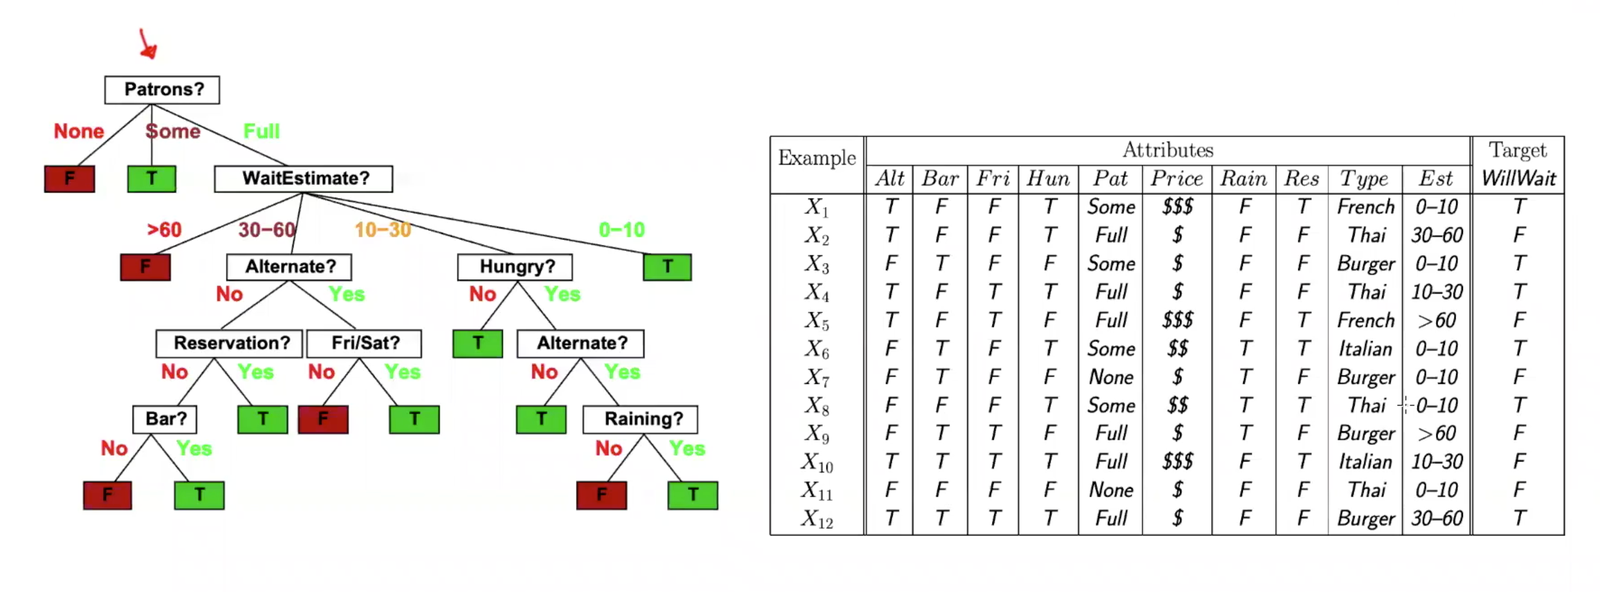
\includegraphics[scale=0.2]{decision1}
	\caption{We have 12 labeled variables}
\end{figure}\end{center}

\noindent This model is called \textbf{\underline{interpretable}} 
	because it is easy to read, as opposed to a neural network.\\
Classifying a variable is as easy as parsing the tree!\\
	\indent Consider $X_{12}$ — we can just walk; this probability happens to match, but it won’t be in general.\\



\noindent The depth of the decision tree is a sign of its complexity.\\
Splitting is as easy as making a choice.\\
Nodes represent attributes.\\
Leaves represent decisions.

\begin{center}\begin{minipage}{0.6\linewidth}
	\begin{figure}[H]
		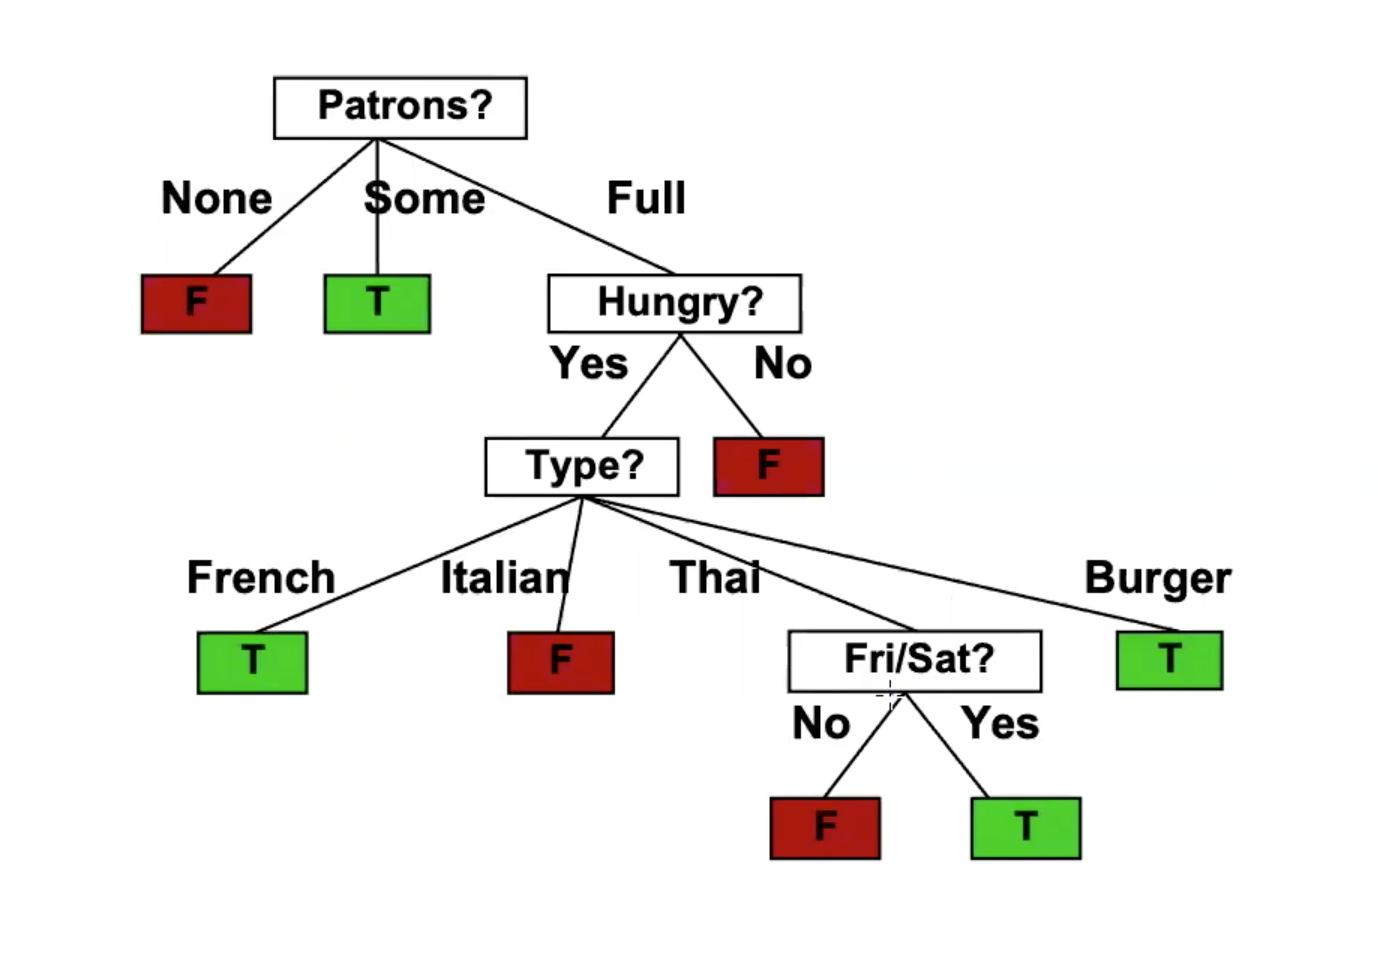
\includegraphics[scale=0.15]{decision2}
	\end{figure}
\end{minipage}%
\begin{minipage}{0.6\linewidth}
We can equivalently build the left:\\
	\indent This has 4 attributes rather than the 10 from above\\
	\indent This is much shallower, and thus simpler
\end{minipage}\end{center}

\begin{minipage}{0.6\linewidth}
The algorithm itself is very simple; \\we just split repeatedly as if tracing the tree.\\
This assumes a black box for choosing variables, \\but developing one is not hard\\
How do we choose which attribute to split on at a given depth?\\
We use conditional entropy as a score to determine our next split.\\
A snapshot of the algorithm is as right.
\end{minipage}%
\begin{minipage}{0.4\linewidth}\begin{tikzpicture}
	\node (A) {A};
	\node[circle, draw, below left =of A, align=center] (L) {+30\\-40};
	\node[below =0.5cm of L, align=center] (TL) {
		\begin{tabular} { | c | c | }\hline M & \\\hline HI & 30/70\\LO & 40/70\\\hline\end{tabular}};
	\node[below =0cm of TL, align=center] {ENT = 0.935};
	\node[circle, draw, below right =of A, align=center] (R) {+20\\-10};
	\node[below =0.5cm of R, align=center] (TR) {
		\begin{tabular} { | c | c | }\hline M & \\\hline HI & 20/30\\LO & 10/30\\\hline\end{tabular}};
	\node[below =0cm of TR, align=center] {ENT = 0.918};
	\node[below =4.5cm of A] {$\implies$ ENT(M|A) = (0.7)(0.985) + (0.3)(0.918) = 0.965};
	\draw [->] (A.south east) -- (R.north west);
	\draw [->] (A.south west) -- (L.north east);
\end{tikzpicture}\end{minipage}

\noindent How do we evaluate an algorithm? We use \textbf{\underline{cross-validation}}.\\
	\indent $\equiv$ split the dataset into 80/20 training/testing data \& repeat to find average score.\\
\\
This can be generalized one more time to a \textbf{\underline{random forest}}.\\
\indent We build a series of trees and majority vote to determine the output.\\
We call this type of method an ensemble learning method.\\

\begin{center}\begin{forest}
	[, phantom
	[ [ [] [] ] [ [] ]]
	[ [ ] [ [] [] ]]
	[ [ [] [] ] [ [] [] ]]
	]
\end{forest}\end{center}

\noindent Suppose we have a dataset of 5 values; we may bootstrap data sets by random choice to get:


\begin{center}\begin{minipage}{0.3\linewidth}\begin{tikzpicture}
	\draw (1, 0) -- (4, 0) -- (4, 3) -- (1, 3) -- cycle;
	\node at (0, 0.5) (5) {5};
	\draw (5.east) -- (1, 0.5);
	\node at (0, 1) (4) {4};
	\draw (4.east) -- (1, 1);
	\node at (0, 1.5) (3) {3};
	\draw (3.east) -- (1, 1.5);
	\node at (0, 2) (2) {2};
	\draw (2.east) -- (1, 2);
	\node at (0, 2.5) (1) {1};
	\draw (1.east) -- (1, 2.5);
\end{tikzpicture}\end{minipage}%
\begin{minipage}{0.3\linewidth}\begin{tikzpicture}
	\draw (1, 0) -- (4, 0) -- (4, 3) -- (1, 3) -- cycle;
	\node at (0, 0.5) (5) {4};
	\draw (5.east) -- (1, 0.5);
	\node at (0, 1) (4) {1};
	\draw (4.east) -- (1, 1);
	\node at (0, 1.5) (3) {3};
	\draw (3.east) -- (1, 1.5);
	\node at (0, 2) (2) {5};
	\draw (2.east) -- (1, 2);
	\node at (0, 2.5) (1) {3};
	\draw (1.east) -- (1, 2.5);
\end{tikzpicture}\end{minipage}%
\begin{minipage}{0.3\linewidth}\begin{tikzpicture}
	\draw (1, 0) -- (4, 0) -- (4, 3) -- (1, 3) -- cycle;
	\node at (0, 0.5) (5) {4};
	\draw (5.east) -- (1, 0.5);
	\node at (0, 1) (4) {2};
	\draw (4.east) -- (1, 1);
	\node at (0, 1.5) (3) {2};
	\draw (3.east) -- (1, 1.5);
	\node at (0, 2) (2) {1};
	\draw (2.east) -- (1, 2);
	\node at (0, 2.5) (1) {2};
	\draw (1.east) -- (1, 2.5);
\end{tikzpicture}\end{minipage}\end{center}

\noindent The count of numbers chosen will be a parameter.\\
We can test the power using the out of bag examples.\\

\subsection*{Bayesian Network Classifiers}
\begin{center}\begin{tikzpicture}
	\node [circle, draw, minimum size = .75cm] (C) {C}
		child {node [circle, draw] {$A_1$} 
			edge from parent}
		child {node [circle, draw] {$A_2$} 
			edge from parent}
		child[missing]
		child {node [circle, draw] {$A_N$} 
			edge from parent};
	\node[below =of C] (c) {};
	\node[right =0.4cm of c] {...};
\end{tikzpicture}\end{center}
\noindent We set a threshold T to classify inputs st 
	\[ C = \left\{ \begin{array}{lr} 
		c & \text{iff } Pr(C|a_1, a_2, ..., a_N) \geq T\\
		\neg c & \text{iff } Pr(C|a_1, a_2, ..., a_N) < T
	\end{array} \right\} \]
\noindent A specific subset of these are called \textbf{\underline{naive}}.\\
These assume the independence of attributes given the parent.
If we interpret the above as naive, then\begin{align*} Pr(c|a_1, a_2, ..., a_N)
	&= \frac {Pr(a_1, a_2, ..., a_N) Pr(c)} {Pr(a_1, a_2, ..., a_N}\\
	&= \frac {Pr(a_1|c) Pr(a_2|c) ... Pr(a_N|c) Pr(c)} 
		{Pr(a_1, a_2, ..., a_N | c) Pr(c) + Pr(a_1, a_2, ..., a_N | \neg c) Pr(\neg c)}\\
	&= \frac {\left[\prod_{i=1}^N Pr(a_i | c)\right] Pr(c)} 
		{Pr(\cap_{i=1}^N a_i | c) Pr(c)  + Pr(\cap_{i=1}^N a_i |\neg c) Pr(\neg c)}
\end{align*}
\noindent We can thus observe this directly from the tree!\\
\\
Traditionally, we want AI to be easily explainable.\\
Consider the following example:\\

\begin{center}\begin{minipage} {0.6\textwidth}\begin{center}\begin{tikzpicture}
	\node[circle, draw] (C) {C};
	\node[circle, draw, below =of C] (N1) {$N_1$};
	\node[circle, draw, right =of N1] (N2) {$N_2$};
	\node[circle, draw, below left =of N1] (S) {S};
	\node[circle, draw, below =of N1] (G) {G};
	\node[circle, draw, below =of N2] (F) {F};
	\node[circle, draw, below right =of N2] (M) {M};
	\draw [->] (C.south) -- (N1.north);
	\draw [->] (N1.east) -- (N2.west);
	\draw [->] (N1.south west) -- (S.north east);
	\draw [->] (N1.south) -- (G.north);
	\draw [->] (N2.south east) -- (M.north west);
	\draw [->] (N2.south) -- (F.north);
\end{tikzpicture}\end{center}\end{minipage}%
\begin{minipage}{0.4\textwidth}\begin{center}\begin{tabular} { | c | c | c | c | c |}\hline
	S & G & F & M & C\\\hline
	- & - & - & - & -\\
	- & - & - & + & +\\
	... & ...  & ... & ... & ...\\
	+ & + & + & + & +\\\hline
\end{tabular}\end{center}\end{minipage}\end{center}\bigskip

\noindent Say we are asked C|\{S=1, G=0, F=1, M=1\}.\\
We might say "yes, because F \& M!", as S \& G are not used.\\
This is called a \textbf{\underline{PI-explanation}}.\\
In actuality, we can make a tractable circuit from this data, which is much power powerful.\\
This, however, is not as interpretable!\\
In the current day, Random Forests < Bayesian Classifiers < Neural Networks.

\end{document}